\section{RANSAC-Based Motion Filtering}

To differentiate static and dynamic objects in the radar point cloud, we use a RANSAC-based approach on the relationship between azimuth angle $\theta$ and radial Doppler velocity $v_d$.

\subsection*{Principle}
Under ideal conditions, static objects exhibit Doppler values consistent with the vehicle's own motion and orientation. 
These values follow a smooth curve when plotted against azimuth. 
Moving objects, however, deviate from this pattern.
RANSAC (Random Sample Consensus) is used to robustly fit a model to the expected Doppler pattern of static objects. 
Points that do not conform to the model are classified as dynamic.

\subsection*{Mathematical Model}

We assume a second-degree polynomial relationship:
\[
v_d = a\theta^2 + b\theta + c
\]

RANSAC fits this model by iteratively:
\begin{itemize}
    \item Sampling minimal subsets of the data,
    \item Fitting the polynomial,
    \item Identifying inliers whose residual error is below a threshold,
    \item Selecting the model with the highest consensus.
\end{itemize}

Let $\mathbf{X}$ be the input azimuth values and $\mathbf{y}$ the Doppler speeds:

\[
\mathbf{X} = \begin{bmatrix} \theta_1 \\ \theta_2 \\ \vdots \\ \theta_n \end{bmatrix}, \quad 
\mathbf{y} = \begin{bmatrix} v_{d1} \\ v_{d2} \\ \vdots \\ v_{dn} \end{bmatrix}
\]

RANSAC estimates polynomial coefficients $\mathbf{w} = [a, b, c]^T$ such that:

\[
\mathbf{y} \approx \Phi(\mathbf{X}) \cdot \mathbf{w}, \quad
\Phi(\mathbf{X}) = 
\begin{bmatrix}
\theta_1^2 & \theta_1 & 1 \\
\theta_2^2 & \theta_2 & 1 \\
\vdots & \vdots & \vdots \\
\theta_n^2 & \theta_n & 1 \\
\end{bmatrix}
\]

\subsection*{Use in Pipeline}

This filtering step occurs after point-wise filtering (e.g., Doppler and range cuts). It outputs:
\begin{itemize}
    \item \textbf{Inliers} – points likely to be static (used in clustering/ICP)
    \item \textbf{Outliers} – likely dynamic, excluded from ego-motion estimation
\end{itemize}

%TODO: Fix image, use one from project.
\begin{figure}[!htbp]
    \centering
    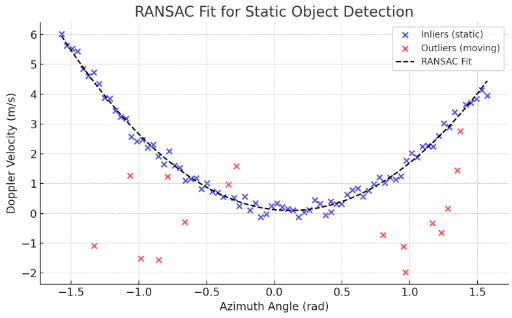
\includegraphics[width=1.0\linewidth]{images/RANSAC.png}
    \caption{RANSAC fit of Doppler vs. azimuth. Inliers = static (blue), Outliers = moving (red). This is simulated data to illustrate the concept.}
    \label{fig:ransac_static_dynamic}
\end{figure}

\subsection{Static vs Dynamic Objects: Role of Doppler}

In radar-based perception, identifying dynamic objects (e.g., vehicles, pedestrians) amidst a cluttered scene of static structures (e.g., walls, poles) is critical.
This task becomes more complex when the radar is mounted on a moving platform, such as a vehicle.
From the sensor's perspective, **all objects appear to move** due to its own motion. The key to resolving this ambiguity lies in leveraging the **Doppler effect**.
The Doppler effect describes how the observed frequency of a wave changes based on the relative motion between the source and the observer. For radar systems, this translates into measurable **radial velocity** values: the component of an object's velocity along the line of sight of the radar.
Assuming the vehicle is moving at a constant speed (e.g., 2 m/s), static targets—such as buildings or parked cars—should exhibit Doppler values that align with this ego-motion, adjusted by their detection angle (azimuth).
That is, a static object located directly ahead will have a Doppler value close to $+2$ m/s (if approaching), while an object at the side (90 azimuth) will have nearly 0 m/s radial velocity.
This expected Doppler pattern for static objects traces a smooth curve when plotted against azimuth. Deviations from this curve indicate potential dynamic objects with their own independent motion.
To robustly extract this pattern from noisy measurements, **RANSAC** is applied to fit a second-order polynomial to the Doppler vs. azimuth data. This model captures the expected distribution of static points.
Points that significantly deviate from this model are considered **dynamic** and excluded from ego-motion estimation steps.

\paragraph{Benefits of RANSAC-Based Filtering:}
\begin{itemize}
    \item Ignores noisy or misdetected points by considering consensus.
    \item Segregates the scene into static (inliers) and dynamic (outliers) segments.
    \item Improves the accuracy of clustering and motion estimation by focusing only on consistent, stationary targets.
\end{itemize}

The filtered result not only enables accurate **object tracking**, but also prevents false ego-motion estimates that could arise from moving targets dominating the point cloud.